\documentclass[12pt]{article}

%%%%%%%%%%%%% GRAPHICS/FONTS
\usepackage{amsmath,amsfonts,graphicx,tikz-cd,pgfplots}

%%%%%%%%%%%%%% FORMATTING
\usepackage{geometry,titlesec,hyperref,xhfill,setspace,float,fancyhdr, parskip}

%%%%%%%%DEFINING COMMANDS
\usepackage{xifthen}

%%%%%%%%%TIKZ STUFF
\usetikzlibrary{positioning,calc}
\usetikzlibrary{decorations.markings}
\usepgfplotslibrary{polar}
\usepgflibrary{shapes.geometric}
\usepgfplotslibrary{fillbetween}

%%%%%%FOR THE GRAPHS
\pgfplotsset{my style/.append style={axis x line=middle, axis y line=
middle, xlabel={$x$}, ylabel={$y$}, axis equal }, compat=1.18}

%%%%%%MARGINS
\geometry{
    letterpaper,
    left=0.5in,
    right=0.5in,
    top=0.5in,
    bottom=0.5in
}

%%%%%%MAKES THE HEADER AND FOOTER FANCY
\fancyhf{}
\renewcommand{\headrulewidth}{0pt}
\pagestyle{fancy}


%%%%%%%%%%%%%%%%%%%%%%
%%%%%%% COMMANDS %%%%%%%
%%%%%%%%%%%%%%%%%%%%%
\newcommand{\underscore}{\underline{\hspace{2mm}}}
\newcommand{\Z}{\mathbb{Z}}
\newcommand{\N}{\mathbb{N}}
\newcommand{\Q}{\mathbb{Q}}
\newcommand{\C}{\mathbb{C}}
\newcommand{\R}{\mathbb{R}}
\newcommand{\Aut}{\text{Aut}}
\newcommand{\GL}{\text{GL}}
\newcommand{\SO}{\text{SO}}
\newcommand{\PGL}{\text{PGL}}
\newcommand{\End}{\text{End}}
\newcommand{\lra}{\longrightarrow}

\newcommand{\RP}{\mathbb{R}P}
\newcommand{\K}{\emph{K}}

\newcommand{\ihat}{\hat{\textbf{i}}}
\newcommand{\jhat}{\hat{\textbf{j}}}

\newcommand{\khat}{\hat{\textbf{k}}}

\newcommand{\abs}[1]{\left\langle #1 \right\rangle}
\newcommand{\qed}{\quad \blacksquare}

%TEXT COMMAND
\newcommand{\T}[1][]{\text{#1}}
\newcommand{\TB}[1][]{\mathbb{#1}}

\newcommand{\xlra}[1][]{%
  \ifthenelse{\isempty{#1}}%
    {\xrightarrow{\phantom{,,,,,,}}}% if #1 is empty
    {\xrightarrow{\phantom{,,}#1\phantom{,,}}}% if #1 is not empty
}



%%%%%%%%%%%%%%%%%%%%%%%%%%%%%%%%%%%%%%%%
%%%%%%%%BEGINNING OF ACTUAL DOCUMENT %%%%%%%%%%
%%%%%%%%%%%%%%%%%%%%%%%%%%%%%%%%%%%%%%%%

%%%%TITLE______REMEMBER TO REGULARLY CHANGE THIS!!!!
\title{Math 1820A Spring 2024 - Homework 1}
\author{}
\date{}

\begin{document}
\maketitle
\vspace{-0.5in}
%%%%%%%%%%%%%%%%

\textbf{Instructions:}  This assignment is worth twenty points.  Please complete the following problems assigned below.  Submissions with insufficient explanation may lose points due to a lack of reasoning or clarity.  If you are handwriting your work, please ensure it is readable and well-formatted for the grader.

Be sure when uploading your work to \textbf{assign problems to pages}.  Problems with pages not assigned to them \textbf{may not be graded}.

\noindent\rule{\textwidth}{1pt}

\textbf{Textbook Problems: }

\noindent\rule{\textwidth}{1pt}

\textbf{Additional Problems:} For these problems, let $e_{i}$ denote the $i$-th coordinate vector in $\R^{n}$. 

\begin{enumerate}
\item Solve the following linear system of differential equations.
\begin{align*}
    \frac{dx_{1}}{dt} &= -2x_{1} + 12x_{2} \\
    \frac{dx_{2}}{dt} &= -x_{1} + 5x_{2} \\
\end{align*}
where $x_{1}(0) = x_{2}(0) = 1$. 

    \color{blue}
        \begin{align*}
            \frac{d}{dt} \begin{pmatrix}
                x_1\\x_2
            \end{pmatrix} &= \begin{pmatrix}
                -2 & 12\\ 
                -1 & 5
            \end{pmatrix} \begin{pmatrix}
                x_1\\ x_2
            \end{pmatrix}\\ 
            &\implies (-2 - \lambda)(5 - \lambda) + 12 = 0\\
            &\implies \lambda^2 - 3\lambda + 2 = 0\\
            &\implies \lambda_1 = 1, \; \lambda_2 = 2\\
            &\implies \begin{pmatrix}
                -2 - \lambda_1 & 12\\ 
                -1 & 5 - \lambda_1
            \end{pmatrix} = \begin{pmatrix}
                -3 & 12\\ 
                -1 & 4
            \end{pmatrix} \implies \begin{cases}
                -3v_1 + 12v_2 = 0\\
                -v_1 + 4v_2 = 0
            \end{cases} \implies v_{\lambda_1} = \begin{pmatrix}
                4\\ 1
            \end{pmatrix}\\
            &\implies \begin{pmatrix}
                -2 - \lambda_2 & 12\\
                -1 & 5 - \lambda_2
            \end{pmatrix} = \begin{pmatrix}
                -4 & 12\\
                -1 & 3
            \end{pmatrix} \implies \begin{cases} 
                -4v_1 + 12v_2 = 0\\
                -v_1 + 3v_2 = 0
            \end{cases} \implies v_{\lambda_2} = \begin{pmatrix}
                3\\ 1
            \end{pmatrix}\\
            \implies x(t) &= C_1 e^{t}\begin{pmatrix}
                4\\ 1
            \end{pmatrix} + C_2 e^{2t} \begin{pmatrix}
                3\\ 1
            \end{pmatrix}\\
            \implies x(0) &= C_1 \begin{pmatrix}
                4\\1
            \end{pmatrix} + C_2 \begin{pmatrix}
                3\\1
            \end{pmatrix} = \begin{pmatrix}
                1\\1
            \end{pmatrix} \implies \implies \begin{cases}
                4C_1 + 3C_2 = 1\\
                C_1 + C_2 = 1
            \end{cases} \implies C_1 = -2, \; C_2 = 3\\ 
            \implies &\boxed{x(t) = -2e^{t}\begin{pmatrix}
                4\\ 1
            \end{pmatrix} + 3e^{2t} \begin{pmatrix} 
                3\\ 1
            \end{pmatrix}}
        \end{align*}
    \color{black}
\pagebreak


\item Draw some trajectories of the linear system in Problem 1. 

\begin{figure}[H]
    \centering
    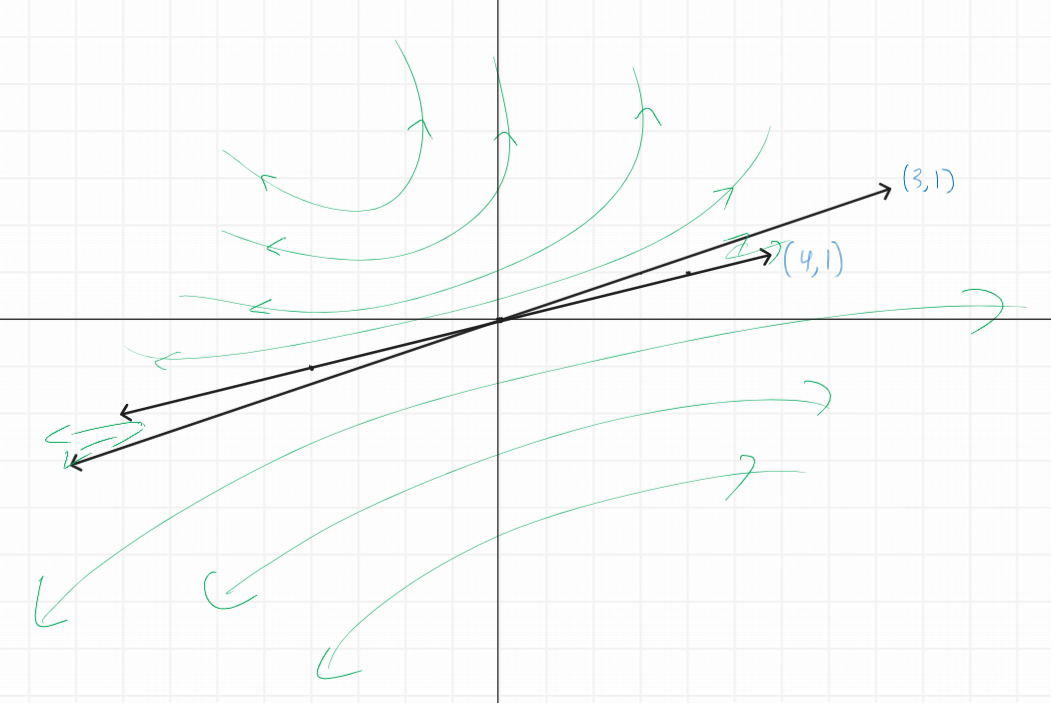
\includegraphics[width=0.8\textwidth]{Images/P2 Trajectories.png}
\end{figure}

\pagebreak

\item Solve the following linear system of differential equations.
\begin{align*}
\frac{dx_{1}}{dt} &= -13x_{1} + 17x_{2} \\
\frac{dx_{2}}{dt} &= -10x_{1} + 13x_{2} \\
\end{align*}
where $x_{1}(0) = x_{2}(0) = 1$.

    \color{blue}
        \begin{align*}
            \frac{d}{dt} \begin{pmatrix}
                x_1\\ x_2
            \end{pmatrix} &= \begin{pmatrix}
                -13 & 17\\ 
                -10 & 13
            \end{pmatrix} \begin{pmatrix}
                x_1\\ x_2
            \end{pmatrix}\\
            &\implies (-13 - \lambda)(13 - \lambda) + 170 = 0 \implies \lambda^2 + 1 =0 \implies \lambda_1 = i, \; \lambda_2 = -i\\ 
            &\implies \begin{pmatrix}
                -13 - \lambda_1 & 17\\ 
                -10 & 13 - \lambda_1
            \end{pmatrix} = \begin{pmatrix}
                -13 - i & 17\\ 
                -10 & 13 - i
            \end{pmatrix} \implies (-13 - i)x_1 + 17x_2 = 0 \\ 
            &\implies v_{\lambda_1} = \begin{pmatrix}
                13 - i\\ 
                10
            \end{pmatrix}\\
            &\implies x(t) = e^{it}\begin{pmatrix}
                13-i\\ 10
            \end{pmatrix} = (\cos(t) + i\sin(t))\left(\begin{pmatrix}
                13\\10
            \end{pmatrix} + i\begin{pmatrix}
                -1\\0
            \end{pmatrix}\right)\\ 
            x(t) &= C_1\begin{pmatrix}
                13\cos(t) + \sin(t)\\ 10\cos(t)
            \end{pmatrix} + C_2\begin{pmatrix}
                13\sin(t) - \cos(t)\\ 10\sin(t)
            \end{pmatrix}\\ 
            \implies x(0) &= C_1 \begin{pmatrix}
                13\\ 10
            \end{pmatrix} + C_2 \begin{pmatrix}
                -1\\ 0
            \end{pmatrix} = \begin{pmatrix}
                1\\1
            \end{pmatrix} \implies \begin{cases}
                13C_1 - C_2 = 1\\
                10C_1 = 1
            \end{cases} \implies C_1 = \frac{1}{10}, \; C_2 = \frac{3}{10}\\    
            \implies x(t) &= \begin{pmatrix}
                \frac{13}{10}\cos(t) + \frac{1}{10}\sin(t) + \frac{39}{10}\sin(t) - \frac{3}{10} \cos(t)\\ 
                \cos(t) + 3\sin(t)
            \end{pmatrix} = \boxed{\begin{pmatrix}
                \cos(t) + 4\sin(t)\\ 
                \cos(t) + 3\sin(t)
            \end{pmatrix}}
       \end{align*}
    \color{black}

\pagebreak
\item Let $A$ be a real 2$\times$2-matrix with non-real complex eigenvalues.  Explain why there exists an invertible matrix $P$ such that 
\[
    A = PRP^{-1} \text{ where } R = r\left(
    \begin{array}{cc}
    \cos(\theta) & -\sin(\theta) \\
    \sin(\theta) & \cos(\theta)
    \end{array}
    \right)
\]
for some $r > 0$ and $\theta \notin 2\pi \Z$ where $r$ and $\theta$ are expressible in terms of the eigenvalues of $A$.

    \color{blue}
       Since $A$ is real, if $\lambda = a + bi$ is an eigenvalue of $A$, then the conjugate $\lambda = a - bi$ is also an eigenvalue of $A$. Then since $A$ has two distinct eigenvalues, it is diagonalizable. Further, its eigenvectors are conjugates.
        
        Since we know its eigenvalues are $a \pm bi$, $A$ is similar to $\begin{pmatrix}
            a & -b\\ 
            b & a
        \end{pmatrix}$. Then, letting $r = \abs{\lambda} = \sqrt{a^2 + b^2}$ and $\theta = \tan^{-1}(\frac{b}{a})$, we have that
        \[\begin{pmatrix}
            a & -b\\ 
            b & a
        \end{pmatrix} = r\begin{pmatrix}
            a/r & -b/r\\ 
            b/r & a/r
        \end{pmatrix} = r\begin{pmatrix}
            \cos(\theta) & -\sin(\theta)\\ 
            \sin(\theta) & \cos(\theta)
        \end{pmatrix}\]
        Call this $R$. Then, $A \sim R$. Equivalently, $A = PRP^{-1}$ for some invertible $P$. 
    
    \color{black}

\pagebreak
\item Let A be a real $2\times 2$-matrix with non-real complex eigenvalues where one of them has real part less than $0$, i.e. $\lambda = a + ib$, where $a < 0$. Let $x_0 \in \R^2$ and define $\gamma_{x_0}(t)$ be the solution to $x' = Ax$ with $\gamma(0) = x_0$. Calculate $\lim_{t \to \infty} \gamma_{x_0}(t)$.
    \color{blue}
        Since $A$ is real and $2 \times 2$, we know that it has two (distinct) eigenvalues which are conjugates of each other. We will make the change of representation $\lambda = -a + bi$ with $a > 0$ (so the other eigenvalue is $-a - bi$). Let $v_1$ be the eigenvector associated with $-a + bi$. Then the solution to the system will be of the form 
        \begin{align*}
            \gamma_{x_0}(t) &= e^{(-a + bi)t} v_1\\ 
                &= e^{-at}e^{bti}v_1\\
                &= e^{-at}(\cos(bt) + i\sin(bt))v_1\\ 
                &= e^{-at} \cos(bt) v_1 + ie^{-a}\sin(bt)v_1
        \end{align*}
        and the general solution will be of the form 
        \[x(t) = C_1e^{-at}\cos(bt) v_1 + C_2e^{-at}\sin(bt)v_1\]
        where $\gamma(0) = x_0 = \begin{pmatrix}
            C_1\\ C_2
        \end{pmatrix}$. 

        Because the exponential argument is negative for both terms, we have that 
        \[\boxed{\lim_{t \to \infty} \gamma_{x_0} = 0}\]

    \color{black}

\pagebreak
\item  Solve the following linear system of differential equations.
\begin{align*}
\frac{dx_{1}}{dt} &= -x_{1}+x_{2}+x_{3} \\
\frac{dx_{2}}{dt} &= -x_{1} + 2x_{2} \\
\frac{dx_{3}}{dt} &= -2x_{1}+5x_{2}-x_{3}
\end{align*}
where $x_{1}(0) = x_{2}(0) = x_{3}(0) = 1$.  (Hint: the characteristic polynomial is $-\lambda^{3}$).  \\

    \color{blue}
        Let $A = \begin{pmatrix}
            -1 & 1 & 1\\
            -1 & 2 & 0\\
            -2 & 5 & -1
        \end{pmatrix}$. Then, we seek to solve $x' = Ax$ with $x(0) = \begin{pmatrix}
            1\\1\\1
        \end{pmatrix}$. 

        Immediately, we see that $x(t) = e^{tA}\begin{pmatrix}
            1\\1\\1
        \end{pmatrix}$.

        Since the characteristic polynomial is $-\lambda^3$, we have that $\lambda = 0$ is an eigenvalue of $A$. But by the Cayley Hamilton Theorem, we also have that $A^3 = 0$. 

        Thus expanding, 
        \[e^{tA} = I + tA + \frac{1}{2}t^2A^2 = \begin{pmatrix}
            1 & 0 & 0\\
            0 & 1 & 0\\
            0 & 0 & 1
        \end{pmatrix} + \begin{pmatrix}
            -t & t & t\\
            -t & 2t & 0\\
            -2t & 5t & -t
        \end{pmatrix} + \frac{1}{2}\begin{pmatrix}
            -2t^2 & 6t^2 & -2t^2\\ 
            -t^2 & 3t^2 & -t^2\\ 
            -t^2 & 3t^2 & -t^2
        \end{pmatrix} = \begin{pmatrix}
           1- t - t^2 & t + 3t^2 & t - t^2\\
           -t - \frac{1}{2}t^2 & 1 + 2t + \frac{3}{2}t^2 & -\frac{1}{2}t^2\\ 
           -2t - \frac{1}{2}t^2 & 5t + \frac{3}{2}t^2 & 1 - t - \frac{1}{2}t^2
        \end{pmatrix}\]
        
        Adding the initial condition, 
        \begin{gather*}
            e^{tA} x_0 = \begin{pmatrix}
                1- t - t^2 & t + 3t^2 & t - t^2\\
                -t - \frac{1}{2}t^2 & 1 + 2t + \frac{3}{2}t^2 & -\frac{1}{2}t^2\\ 
                -2t - \frac{1}{2}t^2 & 5t + \frac{3}{2}t^2 & 1 - t - \frac{1}{2}t^2
            \end{pmatrix} \begin{pmatrix}
                1\\1\\1
            \end{pmatrix}\\
            \boxed{x(t) = \begin{pmatrix}
                1 + t^2\\ 
                1 + t + \frac{1}{2}t^2\\ 
                1 + 2t + \frac{1}{2}t^2 
            \end{pmatrix}}
        \end{gather*}
    \color{black}

\pagebreak
\item Write $x(t) = M(t)x_{0}$ where $M(t)$ is some smooth family of matrices in $\R^{n\times n}$ parametrized by the variable $t$.  What differential equation and initial condition must $M(t)$ satisfy in order for $x(t)$ to be a solution to the linear system $x' = Ax$ for each choice of $x(0) = x_{0}$?  (Hint:  Just plug it in and take derivatives). 

    \color{blue}
        To be a solution to $x' = Ax$, $x(t)$ must itself satisfy the differential equation.  Substituting, 
        \[x' = M'(t)x_0 = Ax(t) = AM(t)x_0 \implies M'(t) = AM(t)\]
        But we also have that $x(0) = x_0$ so $x(0) = M(0)x_0 = x_0$ which implies that $M(0) = I$. Thus, $M(t)$ must satisfy: 
        \[\boxed{M'(t)= AM(t), \quad M(0) = I}\]
    \color{black}

\pagebreak
\item  Let $s(t)$ be a solution to $x' = Ax$ where $A$ is of the form
\[
    A = \left(\begin{array}{ccccc}
    \lambda & 1 & 0 \\
    0 & \lambda & 1 \\
    0 & 0 & \lambda
    \end{array}
    \right)
\]
Let $s_{1}(t) = e^{t\lambda}e_{1}$.  Let $s_{2}(t) = e^{t\lambda}\left(te_{1}+e_{2}\right)$.  Figure out a third solution $s_{3}(t)$ to $x' = Ax$.  (You should think about what this looks like for larger Jordan blocks and how this relates to the Jordan decomposition)

    \color{blue}
        First note that 
        \[A = \begin{pmatrix}
            \lambda & 0 & 0\\ 
            0 & \lambda & 0\\ 
            0 & 0 & \lambda
        \end{pmatrix} + \begin{pmatrix}
            0 & 1 & 0\\ 
            0 & 0 & 1\\ 
            0 & 0 & 0
        \end{pmatrix}\]
        We will denote the diagonal matrix $D$ and the nilpotent matrix $N$. Further note that $ND = DN$ so solving $x' = Ax$ gives 
        \[x(t) = e^{tA}x_0\]
        and 
        \[e^{tA} = e^{t(D + N)} = e^{tD}e^{tN}\] 
        As it is diagonal, $e^{tD}$ is easy:
        \[e^{tD} = \begin{pmatrix}
            e^{\lambda t} & 0 & 0\\ 
            0 & e^{\lambda t} & 0\\ 
            0 & 0 & e^{\lambda t}
        \end{pmatrix}\]

        For $e^{tN}$, we notice that $N^3 = 0$ so 
        \[e^{tN} = I + tN + \frac{1}{2}t^2 N^2 = \begin{pmatrix}
            1 & t & \frac{t^2}{2}\\ 
            0 & 1 & t\\ 
            0 & 0 & 1
        \end{pmatrix}\]
        
        Thus,
        \[e^{tA} = \begin{pmatrix}
            e^{\lambda t} & 0 & 0\\ 
            0 & e^{\lambda t} & 0\\ 
            0 & 0 & e^{\lambda t}
        \end{pmatrix} \begin{pmatrix}
            1 & t & \frac{t^2}{2}\\ 
            0 & 1 & t\\ 
            0 & 0 & 1
        \end{pmatrix} = e^{t\lambda} \begin{pmatrix}
            1 & t & \frac{t^2}{2}\\ 
            0 & 1 & t\\ 
            0 & 0 & 1
        \end{pmatrix}\]

        Now to get the third column, we introduce the initial condition $x_0 = \begin{pmatrix}
            0\\0\\1
        \end{pmatrix}$, 
        \begin{align*}
            s_3(t) &= e^{tA}x_0\\ 
                &= e^{t\lambda}\begin{pmatrix}
                1 & t & \frac{t^2}{2}\\ 
                0 & 1 & t\\ 
                0 & 0 & 1
            \end{pmatrix} \begin{pmatrix}
                0\\0\\1
            \end{pmatrix}\\ 
            &= \boxed{e^{t\lambda} (\frac{t^2}{2}e_1 + te_2 + e_3)}
        \end{align*}
    \color{black}
\end{enumerate}
\end{document}